\sidefig*(75mm){
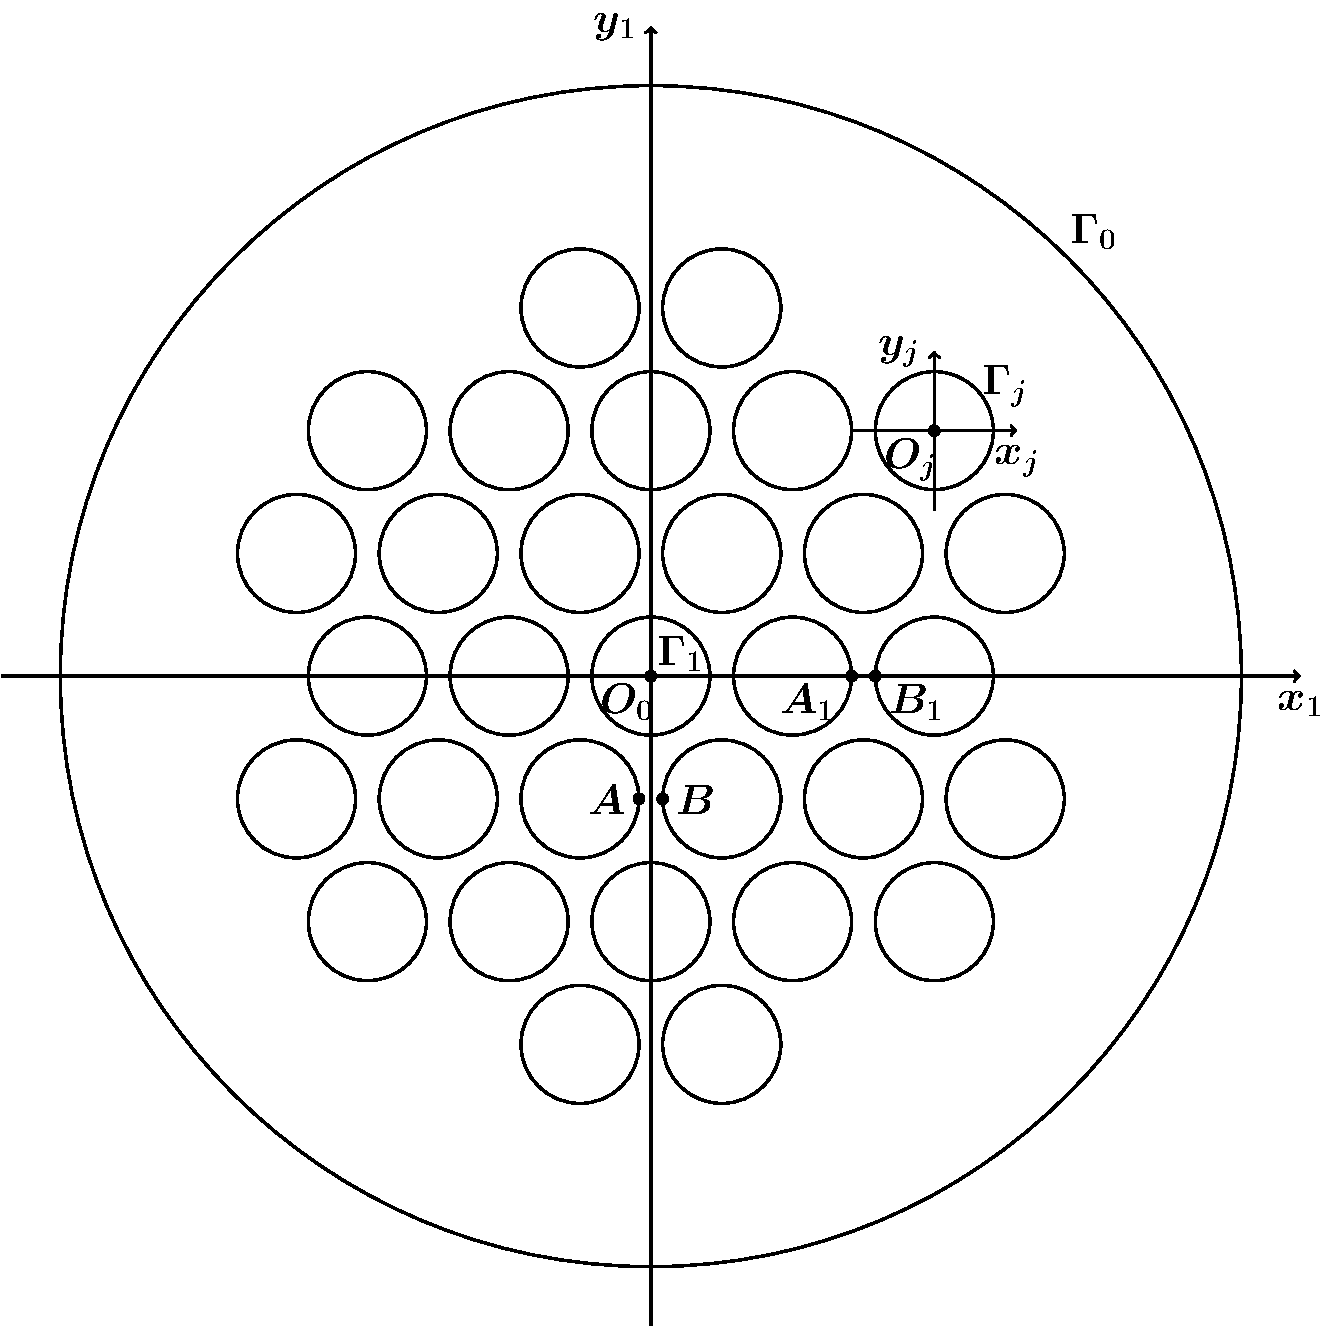
\includegraphics[width=7.5cm]{hexagonal-centroid.pdf}
\caption{Гексагональная центрированная структура расположения полостей в цилиндрическом образце}
\label{f:7:24}
}{Текст текст текст текст текст текст текст текст текст текст текст текст текст текст текст текст текст текст текст текст текст текст текст текст текст текст текст текст текст текст текст текст текст текст текст текст текст текст текст текст текст текст текст текст текст текст текст текст текст текст текст текст текст текст текст текст текст текст текст текст текст текст текст текст текст текст текст текст текст текст текст текст текст текст текст текст текст текст текст текст текст текст текст текст текст текст текст текст текст текст текст текст текст текст текст текст текст текст текст}

\begin{figure}[h!]
\centering\footnotesize
\parbox[b]{7.5cm}{\centering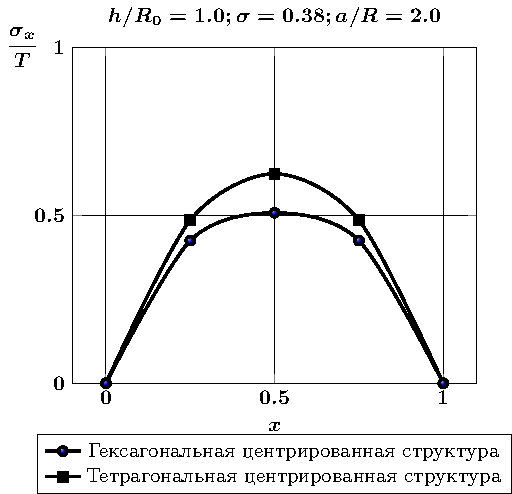
\includegraphics[width=7.5cm]{cav7-5-sig_x.pdf}
\caption{Относительные напряжения $\sigma_x/T$ на линии, соединяющей центры соседних полостей для гексагональной и тетрагональной центрированных структур
\label{f:7:25}}}\hfil\hfil
\parbox[b]{7.5cm}{\centering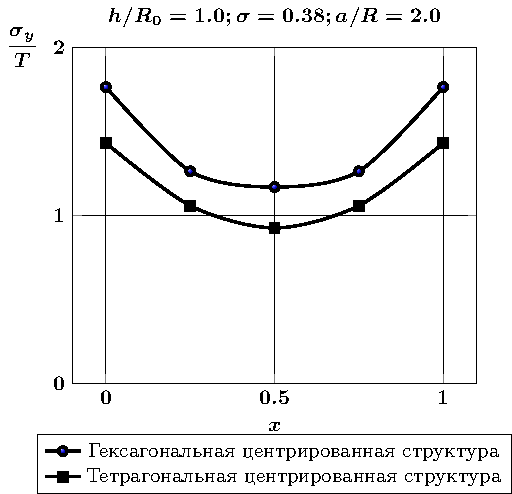
\includegraphics[width=7.5cm]{cav7-5-sig_y.pdf}
\caption{Относительные напряжения $\sigma_y/T$ на линии, соединяющей центры соседних полостей для гексагональной и тетрагональной центрированных структур
\label{f:7:26}}}
\end{figure}

legend style={anchor=north,legend columns=2},